\documentclass[a4paper]{article}

\usepackage[portuguese,english]{babel}
\usepackage[utf8]{inputenc}
\usepackage[T1]{fontenc}

\newcommand{\documentTitle}{Data Analysis and Transformation \\ TP3: Sampling Theorem, Discrete Fourier Transform and Audio and Image Signals' Filtering}
\newcommand{\pdfTitle}{[ATD] TP3: Sampling Theorem, Discrete Fourier Transform and Audio and Image Signals' Filtering}
\newcommand{\documentAuthors}{José Ribeiro (2008112181, jbaia@student.dei.uc.pt) \\ Pedro Magalhães (2009117002, pjrosa@student.dei.uc.pt)}

\title{\documentTitle}
\author{\documentAuthors}

\usepackage{hyperref}
\hypersetup{
	pdftitle = \pdfTitle
	,pdfauthor = \documentAuthors
	,pdfsubject = {Data Analysis and Transformation}
	,pdfkeywords = {Data Analysis and Transformation} {Sampling Theorem} {Discrete Fourier Transform}
	,pdfborder = {0 0 0}
}

%\usepackage{subfig}
%\usepackage{amsmath}
%\usepackage{array}
\usepackage{anysize}
\usepackage{lscape}
\usepackage{amsmath}
\usepackage{graphicx}
\usepackage{caption}
\usepackage{amssymb}
%\usepackage[pdftex]{graphicx}
%\usepackage[table]{xcolor}

\hyphenation{}

\marginsize{2.3cm}{2.3cm}{3cm}{3cm}

\makeatletter

\begin{document}
\maketitle
\cleardoublepage

\tableofcontents
\cleardoublepage

\setlength{\parindent}{1cm}
\setlength{\parskip}{0.3cm}

\section{Exercise 1}
\subsection{Exercise 1.1}
\label{subsec:ex_1_1}
\noindent Após a substituição do número de grupo na fórmula, procedeu-se à sua simplificação segundo a forma de Série de Fourier.
\begin{eqnarray}
	x(t) & = & -1 + 3 \, sin(30 \, \pi \, t) + 4 \, sin\left( 12 \, \pi \, t - \frac{\pi}{4} \right) \, cos(21 \, \pi \, t) \\
	& = & cos(\pi) + 3 \, cos\left( 30 \, \pi \, t - \frac{\pi}{2} \right) + 2 \, \left( sin\left( \left( 12 \, \pi \, t - \frac{\pi}{4} \right) + 21 \, \pi \, t \right) + sin\left( \left( 12 \, \pi \, t - \frac{\pi}{4} \right) - 21 \, \pi \, t\right) \right) \\
	& = & cos(\pi) + 3 \, cos\left( 30 \, \pi \, t - \frac{\pi}{2} \right) + 2 \, sin\left( 33 \, \pi \, t - \frac{\pi}{4} \right) + 2 \, sin\left( -9 \, \pi \, t - \frac{\pi}{4} \right) \\
	& = & cos(\pi) + 3 \, cos\left( 30 \, \pi \, t - \frac{\pi}{2} \right) + 2 \, cos\left( 33 \, \pi \, t - \frac{\pi}{4} - \frac{\pi}{2} \right) + 2 \, cos\left( -9 \, \pi \, t - \frac{\pi}{4} - \frac{\pi}{2} \right) \\
	& = & cos(\pi) + 3 \, cos\left( 30 \, \pi \, t - \frac{\pi}{2} \right) + 2 \, cos\left( 33 \, \pi \, t - \frac{3 \, \pi}{4} \right) + 2 \, cos\left( -9 \, \pi \, t - \frac{3 \, \pi}{4} \right) \\
	& = & 1 \, cos(0 \, t + \pi) + 2 \, cos\left( 9 \, \pi \, t + \frac{3 \, \pi}{4} \right) + 3 \, cos\left( 30 \, \pi \, t + \frac{3 \, \pi}{2} \right) + 2 \, cos\left( 33 \, \pi \, t + \frac{5 \, \pi}{4} \right)
\end{eqnarray}

\noindent Com a fórmula nesta forma tornam-se evidentes a frequência fundamental e a frequência máxima. A frequência angular fundamental ($\omega_0$) é dada pelo máximo divisor comum entre as várias frequências angulares, i. e.,
\begin{equation}
	\omega_0 = mdc \, (0, 9 \, \pi, 30 \, \pi, 33 \, \pi) = 3 \, \pi
\end{equation}

\noindent Obtêm-se assim também os valores de
\begin{equation}
	f_0 = \frac{\omega_0}{2 \, \pi} = \frac{3}{2} Hz
\end{equation}

\noindent e
\begin{equation}
	T_0 = \frac{1}{f_0} = \frac{2}{3} s
\end{equation}

\noindent A frequência angular máxima ($\omega_{max}$) é a máxima de todas as frequências angulares, pelo que
\begin{equation}
	\omega_{max} = max \, (0, 9 \, \pi, 30 \, \pi, 33 \, \pi) = 33 \, \pi
\end{equation}

\noindent Segundo o Teorema de Nyquist-Shannon, para que um sinal possa ser reconstruído sem erro a partir de uma sequência resultante da sua amostragem, a frequência de amostragem utilizada deverá ser superior ao dobro da maior frequência presente no sinal original, ou seja,
\begin{equation}
	f_s > 2 \, f_{max}
\end{equation}

\noindent De forma a garantir que a frequência de amostragem escolhida obedece à condição e é um múltiplo da frequência fundamental,
\begin{equation}
	f_s = 2 \, f_{max} + n \, f_0, ~ n \in \mathbb{N}
\end{equation}

\noindent dado que $f_{max}$ é múltiplo de $f_0$. Aplicando esta fórmula a frequências angulares,
\begin{equation}
	w_s = 2 \, w_{max} + n \, w_0, ~ n \in \mathbb{N}
\end{equation}

\noindent Escolheu-se $n = 2$ dado que, como $w_0$ e $w_{max}$ são múltiplos de $\pi$, $w_s$ será múltipla de $2 \, \pi$, o que garante que a sua conversão de $radianos$ para $hertz$ dará um número inteiro. Conclui-se que
\begin{equation}
	w_s = 2 * 33 \, \pi + 2 * 3 \, \pi = 72 \, \pi \, rad/s
\end{equation}

\noindent e consequentemente
\begin{equation}
	f_s = \frac{w_s}{2 \, \pi} = \frac{72 \, \pi}{2 \, \pi} = 36 \, Hz
\end{equation}

\begin{equation}
	T_s = \frac{1}{f_s} = \frac{1}{36} \, s
\end{equation}

\noindent A expressão de $x[n]$ é, consequentemente,
\begin{eqnarray}
	x[n] = x(t)|_{t = n \, T_s} = & cos(\pi) + 2 \, cos\left( 9 \, \pi \, n \, T_s + \frac{3 \, \pi}{4} \right) + 3 \, cos\left( 30 \, \pi \, n \, T_s + \frac{3 \, \pi}{2} \right) + 2 \, cos\left( 33 \, \pi \, n \, T_s + \frac{5 \, \pi}{4} \right) \\
	= & cos(\pi) + 2 \, cos\left( \frac{9 \, \pi}{36} \, n + \frac{3 \, \pi}{4} \right) + 3 \, cos\left( \frac{30 \, \pi}{36} \, n + \frac{3 \, \pi}{2} \right) + 2 \, cos\left( \frac{33 \, \pi}{36} \, n + \frac{5 \, \pi}{4} \right) \\
	= & cos(\pi) + 2 \, cos\left( \frac{\pi}{4} \, n + \frac{3 \, \pi}{4} \right) + 3 \, cos\left( \frac{5 \, \pi}{6} \, n + \frac{3 \, \pi}{2} \right) + 2 \, cos\left( \frac{11 \, \pi}{12} \, n + \frac{5 \, \pi}{4} \right)
\end{eqnarray}

\subsection{Exercise 1.2}
\noindent Abaixo apresenta-se o sinal de tempo contínuo (i.e., com 5000 pontos) a azul, sobreposto pelo sinal amostrado, a pontos vermelhos.
\begin{center}
	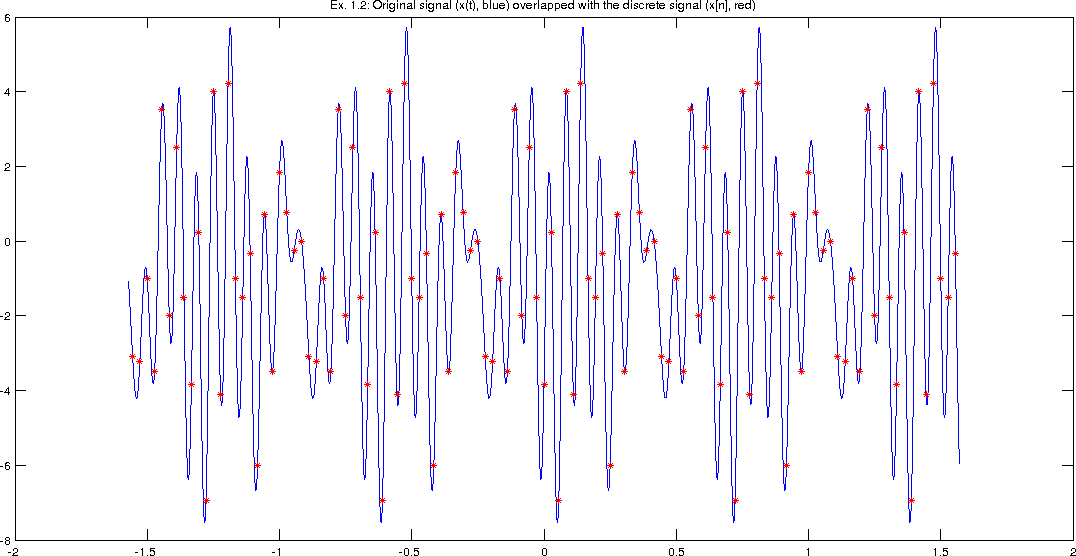
\includegraphics[width=0.70\textwidth]{images/ex_1_2.png}
	\captionof{figure}{Original signal (x(t), blue) overlapped with the discrete signal (x[n], red)}
	\label{fig:ex_1_2}
\end{center}

\noindent Como é possível verificar, todos os pontos vermelhos assentam sobre a curva azul do sinal original.
\clearpage

\subsection{Exercise 1.3}
\noindent Após a utilização das funções \texttt{fft} e \texttt{fftshift}, obtiveram-se os gráficos que de seguida se apresentam (em cima a representação em módulo do resultado da DFT, em baixo a representação em fase).
\begin{center}
	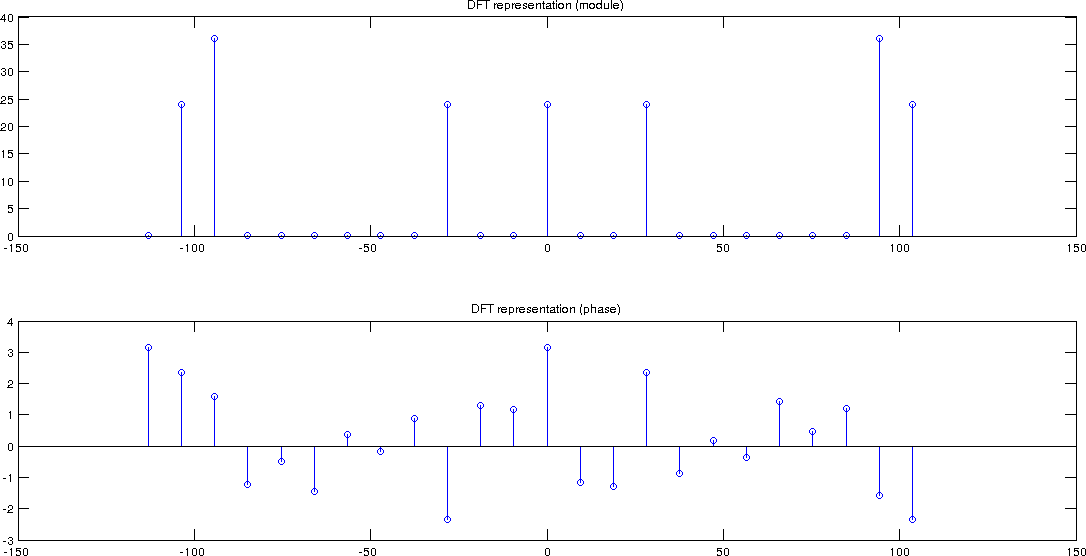
\includegraphics[width=0.70\textwidth]{images/ex_1_3.png}
	\captionof{figure}{DFT representation (above: module; below: phase).}
	\label{fig:ex_1_3}
\end{center}

\subsection{Exercise 1.4}
\label{subsec:ex_1_4}
\noindent A relação entre os coeficientes da Série de Fourier Complexa com a Transformada Discreta de Fourier é dada por
\begin{equation}
	c_m = \frac{1}{N} \, X[m]
\end{equation}

\noindent onde $X$ é o resultado da DFT e N dado por
\begin{equation}
	N = \frac{T_0}{T_s} = \frac{\frac{2}{3}}{\frac{1}{36}} = 24
\end{equation}
\clearpage

\noindent Como tal, é possível obter os coeficientes da Série de Fourier Complexa dividindo o resultado por $N$, o que nos dá o resultado abaixo apresentado (em cima a representação em módulo dos coeficientes, em baixo a representação em fase).

\begin{center}
	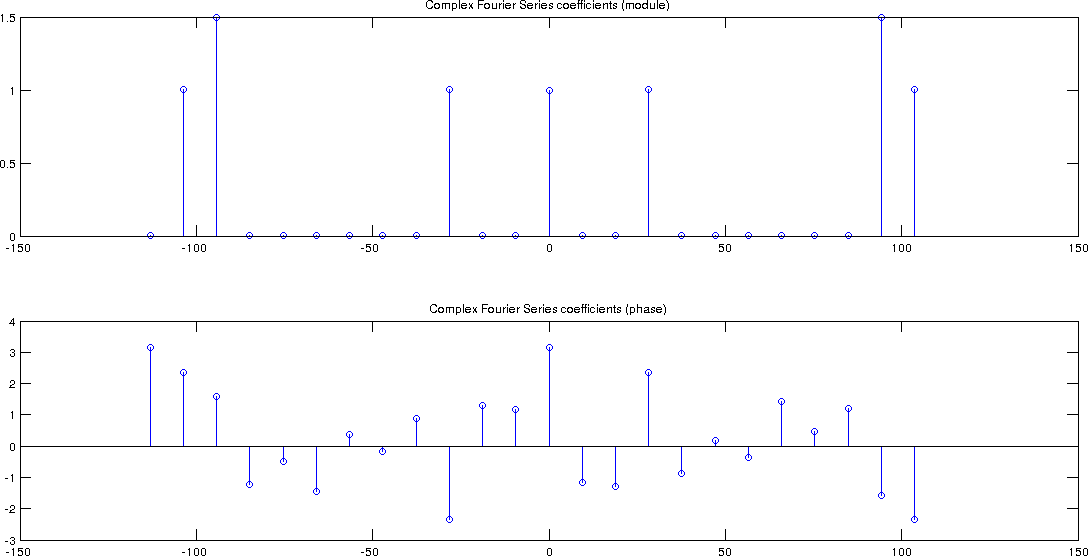
\includegraphics[width=0.70\textwidth]{images/ex_1_4.png}
	\captionof{figure}{Complex Fourier Series coefficients (above: module; below: phase).}
	\label{fig:ex_1_4}
\end{center}

\subsection{Exercise 1.5}
\label{subsec:ex_1_5}
\noindent A partir dos coeficientes da Série de Fourier Complexa é possível obter os coeficientes da Série de Fourier Trigonométrica, com a sua relação dada segundo
\begin{equation}
	c_m = \left\{
	\begin{array}{lr}
		C_0 \, cos(\theta_0) & m = 0 \\
		\, & \, \\
		\frac{C_m}{2} \, (cos~\theta_m + sgn(m)~j~sin~\theta_m), & m \neq 0
	\end{array}
	\right.
	\label{eq:complex_trig_rel}
\end{equation}

\noindent Como tal, e dado que
\begin{equation}
	|cos~\theta_m \pm~j~sin~\theta_m| = 1
\end{equation}

\noindent o valor em módulo de $C_m$ pode ser obtido multiplicando por 2 o valor em módulo de $c_m$, com a excepção do valor de $m = 0$.

\clearpage

\noindent Como o número de coeficientes do lado positivo pode ser menor que o número de coeficientes do lado negativo (consoante a paridade de $N$), optámos por utilizar os Coeficientes da Série de Fourier Complexa do lado negativo para calcular os Coeficientes da Série de Fourier Trigonométrica; como tal, o valor de $\theta_m$ é obtido a partir do conjugado\footnote{Isto porque, segundo a equação \ref{eq:complex_trig_rel}, os $c_m$ correspondentes a $m$ positivo são os valores conjugados dos valores para $m$ negativo.} do valor do ângulo do coeficiente complexo. Apresenta-se agora a representação gráfica (em cima, $C_m$, em baixo, $\theta_m$).
\begin{center}
	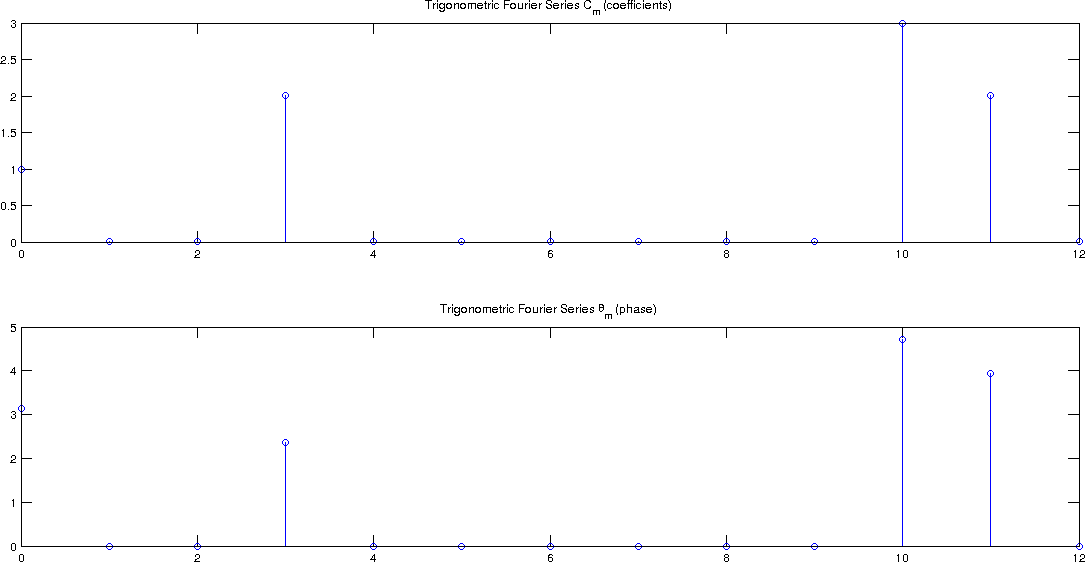
\includegraphics[width=0.70\textwidth]{images/ex_1_5.png}
	\captionof{figure}{Trigonometric Fourier Series parameters ($C_m$ (coefficients, above) and $\theta_m$ (phase, below).}
	\label{fig:ex_1_5}
\end{center}

\clearpage

\subsection{Exercise 1.6}
\noindent Reconstruindo o sinal utilizando a fórmula da Série de Fourier Trigonométrica, isto é,
\begin{equation}
	x(t) = \sum_{i} C_{i} \, cos(\omega_{i} t + \theta_{i})
\end{equation}

\noindent obtivemos o gráfico que abaixo se apresenta (a azul, o sinal original, a vermelho, a reconstrução do sinal).
\begin{center}
	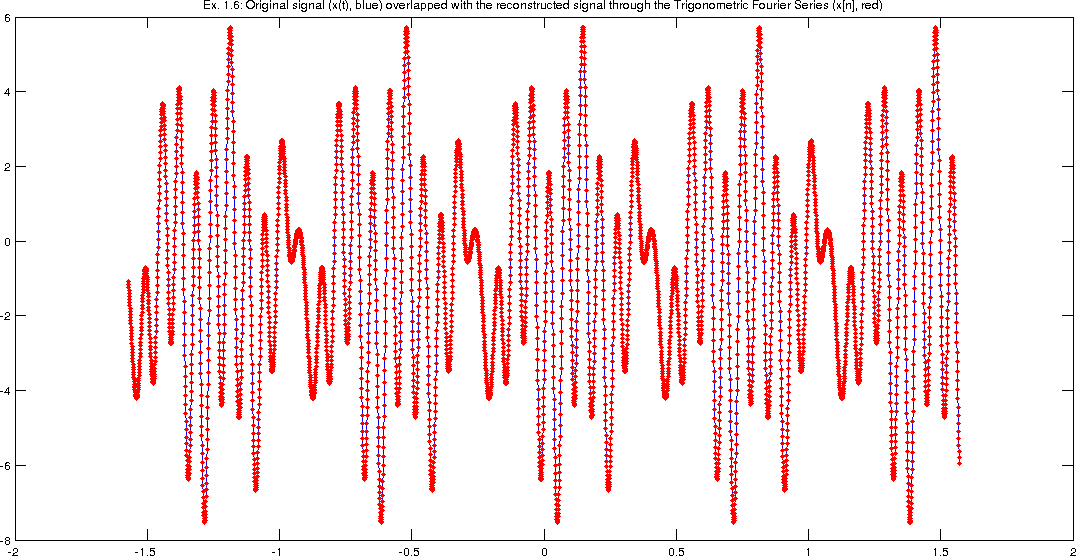
\includegraphics[width=0.70\textwidth]{images/ex_1_6.png}
	\captionof{figure}{Original signal ($x(t)$, blue) overlapped with the reconstructed signal through the Trigonometric Fourier Series ($x[n]$, red)}
	\label{fig:ex_1_6}
\end{center}

\clearpage
\section{Exercise 2}
\subsection{Exercise 2.1}
\noindent Após a utilização das funções \texttt{fft} e \texttt{fftshift}, obtém-se (a partir do módulo da DFT) o espectro do sinal.
\begin{center}
	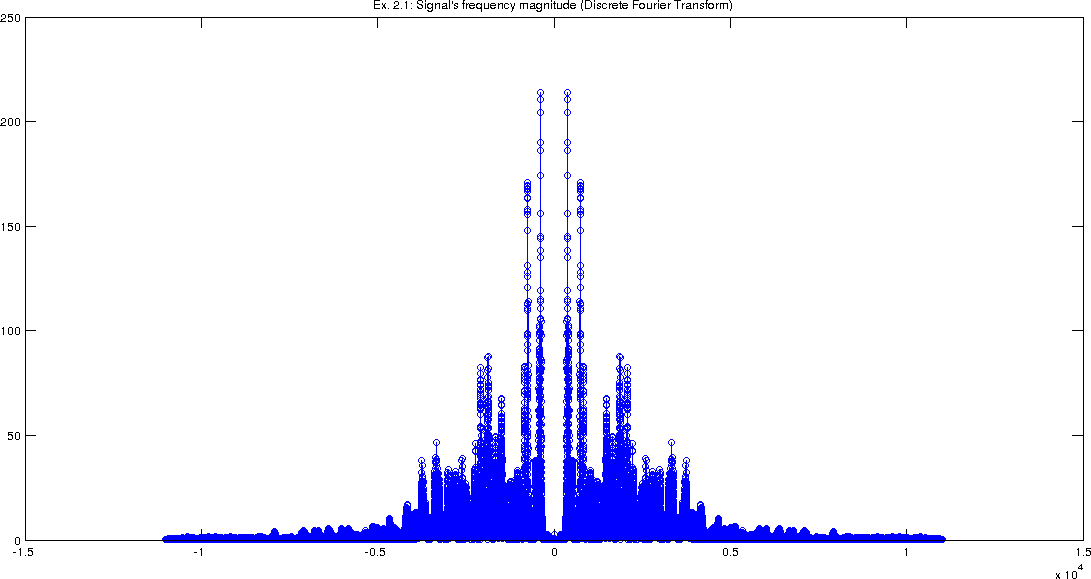
\includegraphics[width=0.70\textwidth]{images/ex_2_1.png}
	\captionof{figure}{Signal's frequency magnitude (Discrete Fourier Transform).}
	\label{fig:ex_2_1}
\end{center}

\subsection{Exercise 2.2}
\noindent A frequência de amplitude máxima é 374.48Hz, com uma amplitude de 0.01. Esta amplitude foi calculada utilizando a relação entre a DFT e a Série de Fourier Trigonométrica, mencionada em \emph{\nameref{subsec:ex_1_4}} e \emph{\nameref{subsec:ex_1_5}}.

\clearpage

\subsection{Exercise 2.3}
\noindent Após o cálculo dos indíces correspondentes à gama a modificar (bem como 10\% da amplitude máxima do espectro), é gerado ruído em amplitude e fase e adicionado a esses mesmos índices. Pela mesma razão que em \emph{\nameref{subsec:ex_1_5}}, existe o cuidado de colocar o conjugado do ruído nos índices do lado negativo. Apresenta-se agora o espectro do sinal original (a azul) sobreposto com o espectro do sinal após a adição de ruído (a vermelho). É possível observar, consequentemente, a gama (a vermelho) onde foi adicionado.
\begin{center}
	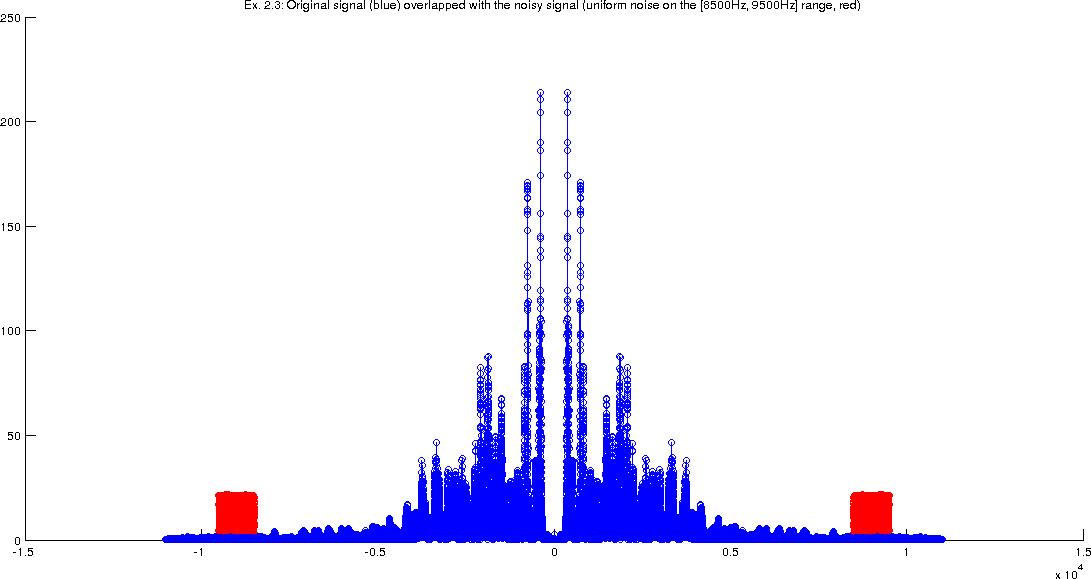
\includegraphics[width=0.70\textwidth]{images/ex_2_3_lowpass.png}
	\captionof{figure}{Original signal (blue) overlapped with the noisy signal (uniform noise on the [8500Hz, 9500Hz] range, red).}
	\label{fig:ex_2_3}
\end{center}

\subsection{Exercise 2.4}
\noindent Após a aplicação de \texttt{ifft} (e \texttt{ifftshift}), o som obtido possui um ruído agudo de fundo (semelhante a "grilos").

\subsection{Exercise 2.5}
\noindent Após a utilização da função \texttt{butter}, cria-se um filtro do tipo Butterworth de ordem 6, com a função de transferência
\begin{equation}
G(z) = \frac{0.1765~z^6 + 1.0589~z^5 + 2.6473~z^4 + 3.5298~z^3 + 2.6473~z^2 + 1.0589~z + 0.1765}{z^6 + 2.6863~z^5 + 3.5022~z^4 + 2.6179~z^3 + 1.1677~z^2 + 0.2901~z + 0.0312}
\end{equation}

\noindent com os zeros \[-1.0048, -1.0024 + i0.0042, -1.0024 - i0.0042, -0.9976 + i0.0042, -0.9976 - i0.0042, -0.9952\] e pólos \[-0.5440 + i0.6129, -0.5440 - i0.6129, -0.4236 + i0.3493, -0.4236 - i0.3493, -0.3756 + i0.1134, -0.3756 - i0.1134\]

\clearpage

\noindent Apresentam-se em seguida no plano Z.
\begin{center}
	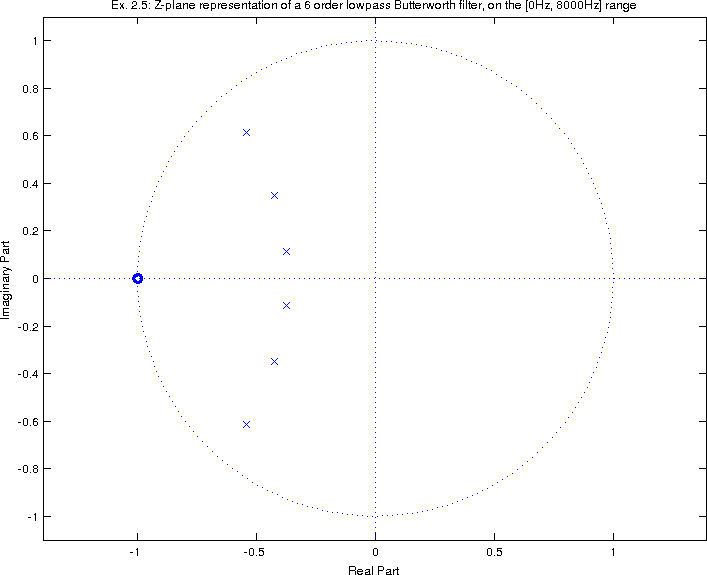
\includegraphics[width=0.70\textwidth]{images/ex_2_5_lowpass_zplane.png}
	\captionof{figure}{Z-plane representation of a 6th order Lowpass Butterworth filter, on the [0Hz, 8000Hz] range.}
	\label{fig:ex_2_5_lowpass_zplane}
\end{center}

\noindent Após a aplicação da função \texttt{filter} sobre o sinal com ruído, obteve-se o seguinte espectro de magnitude para esse sinal filtrado.
\begin{center}
	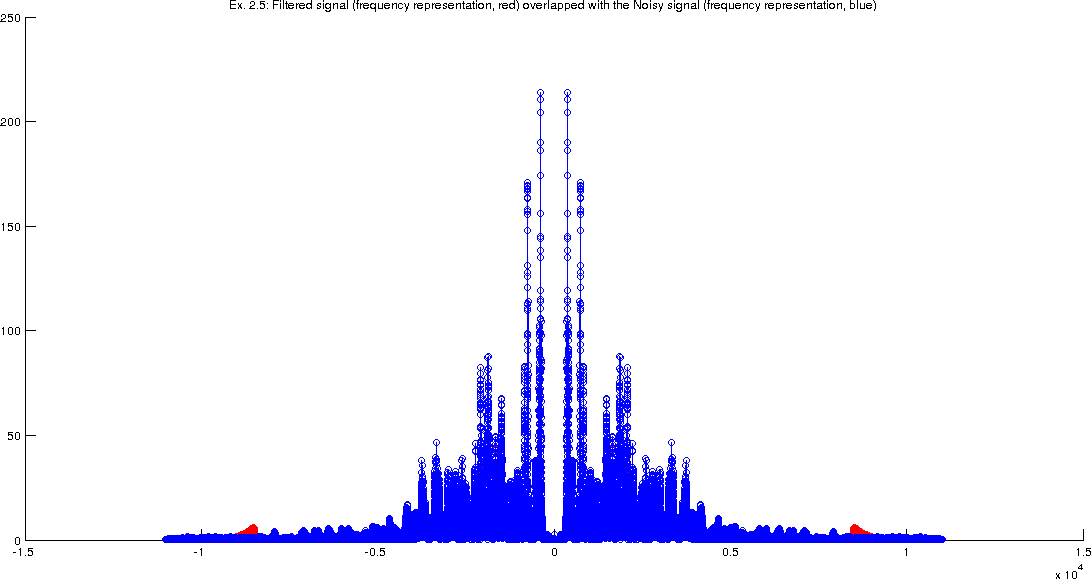
\includegraphics[width=0.70\textwidth]{images/ex_2_5_lowpass_spectrum.png}
	\captionof{figure}{Noisy signal magnitude spectrum, after applying a 6th order Lowpass Butterworth filter, on the [0Hz, 8000Hz] range.}
	\label{fig:ex_2_5_lowpass_spectrum}
\end{center}

\noindent É possível observar uma redução considerável do ruído, em termos de magnitude; o sinal aproxima-se bastante do original.

\subsection{Exercise 2.6}
\noindent Apresentam-se agora as 3 alíneas anteriores, desta vez para ruído na gama $[2000Hz, 3000Hz]$.
\begin{center}
	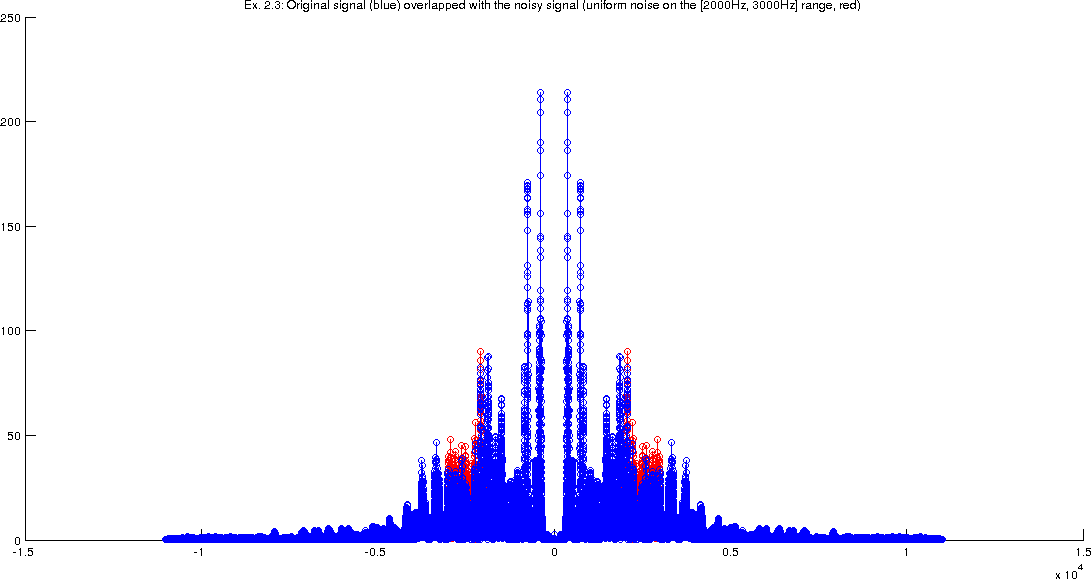
\includegraphics[width=0.70\textwidth]{images/ex_2_3_bandstop.png}
	\captionof{figure}{Original signal (blue) overlapped with the noisy signal (uniform noise on the [2000Hz, 3000Hz] range, red).}
	\label{fig:ex_2_3_bandstop}
\end{center}

\noindent Após a aplicação de \texttt{ifft} (e \texttt{ifftshift}), o som obtido possui um ruído de altura média de fundo (algo oscilatório). \\
\noindent Utiliza-se também um filtro do tipo Butterworth de ordem 6, com a função de transferência
\begin{equation}
G(Z) = \frac{0.7513~z^6 - 3.4465~z^5 + 7.5241~z^4 - 9.5793~z^3 + 7.5241~z^2 - 3.4465~z + 0.7513}{z^6 - 4.1530~z^5 + 8.2060~z^4 - 9.4847~z^3 + 6.7803~z^2 - 2.8346~z + 0.5645}
\end{equation}

\noindent com os zeros \[0.7646 + i0.6446, 0.7646 - i0.6446, 0.7646 + i0.6446, 0.7646 - i0.6446, 0.7645 + i0.6445, 0.7645 - i0.6445\] e pólos \[0.6217 + i0.6810, 0.6217 - i0.6810, 0.7862 + i0.5178, 0.7862 - i0.5178, 0.6686 + i0.5496, 0.6686 - i0.5496\]

\clearpage

\noindent Apresentam-se em seguida no plano Z.
\begin{center}
	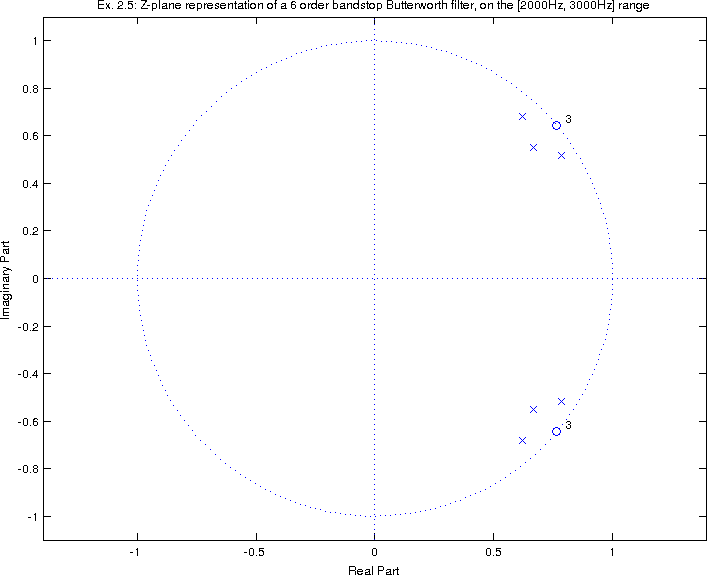
\includegraphics[width=0.70\textwidth]{images/ex_2_5_bandstop_zplane.png}
	\captionof{figure}{Z-plane representation of a 6th order Bandstop Butterworth filter, on the [2000Hz, 3000Hz] range.}
	\label{fig:ex_2_5_bandstop_zplane}
\end{center}

\clearpage

\noindent Após a aplicação da função \texttt{filter} sobre o sinal com ruído, obteve-se o seguinte espectro de magnitude para esse sinal filtrado.
\begin{center}
	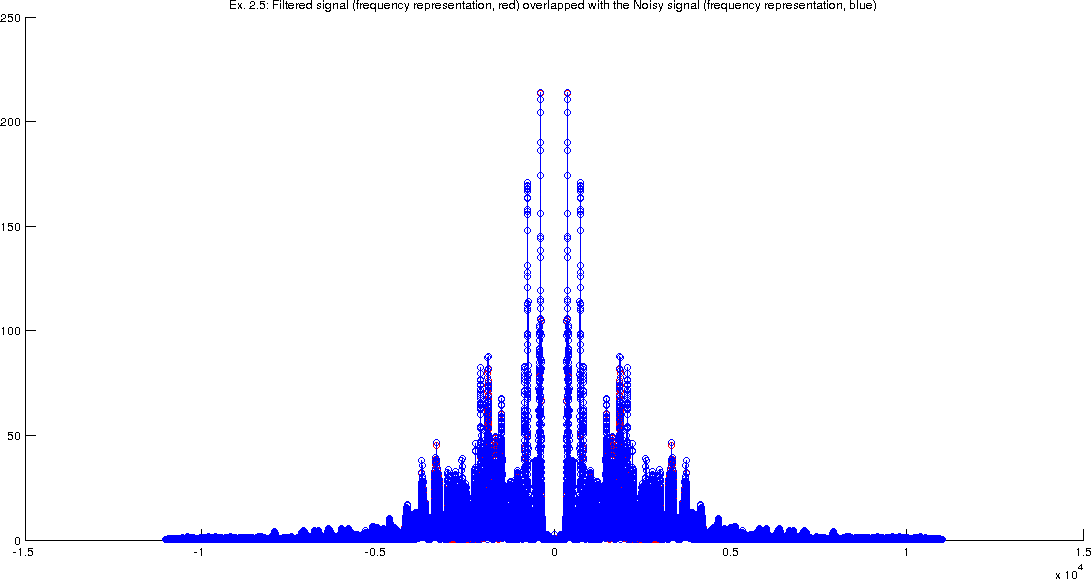
\includegraphics[width=0.70\textwidth]{images/ex_2_5_bandstop_spectrum.png}
	\captionof{figure}{Noisy signal magnitude spectrum, after applying a 6th order Bandstop Butterworth filter, on the [2000Hz, 3000Hz] range.}
	\label{fig:ex_2_5_bandstop_spectrum}
\end{center}

\noindent É possível observar uma redução considerável do ruído, em termos de magnitude. No entanto, nota-se que o saxofone não tem o timbre original. Isto vai de encontro ao esperado, visto este ruído se encontrar numa gama de frequências importantes.

\clearpage

\section{Exercise 3}
\subsection{Exercise 3.1/3.2}
\noindent Apresenta-se a imagem a estudar.
\begin{center}
	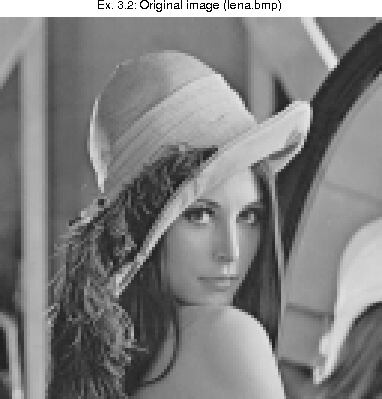
\includegraphics[width=0.20\textwidth]{images/ex_3_2.png}
	\captionof{figure}{Original image (lena.bmp).}
	\label{fig:ex_3_2}
\end{center}

\subsection{Exercise 3.3}
\noindent Em seguida apresenta-se o espectro da imagem, em magnitude.
\begin{center}
	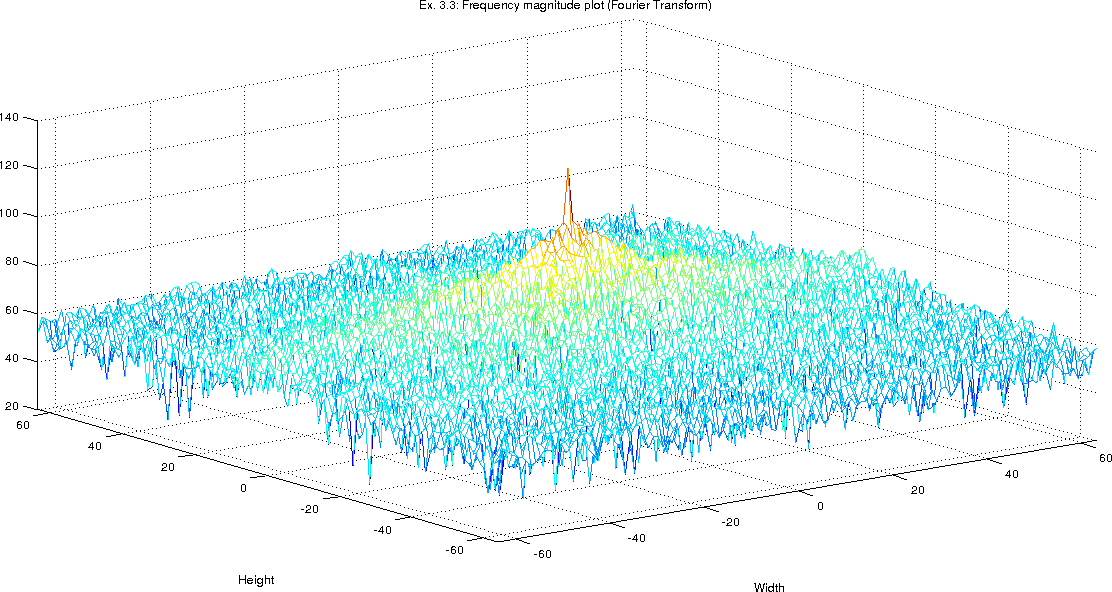
\includegraphics[width=0.70\textwidth]{images/ex_3_3.png}
	\captionof{figure}{Frequency magnitude plot (after the Discrete Fourier Transform).}
	\label{fig:ex_3_3}
\end{center}

\noindent A cor média corresponde à componente $DC$, i.e., à frequência $0$. Como tal, após o cálculo dos índices na matriz da DFT (que antes de aplicar \texttt{fftshift} é $(1,1)$) correspondentes a essa componente, tem-se que a amplitude aproximada é de $124.3$.

\clearpage

\subsection{Exercise 3.4 - Exercise 3.8}
\noindent Apresenta-se em seguida a máscara criada para um filtro passa-baixo, de frequência de corte $20$.
\begin{center}
	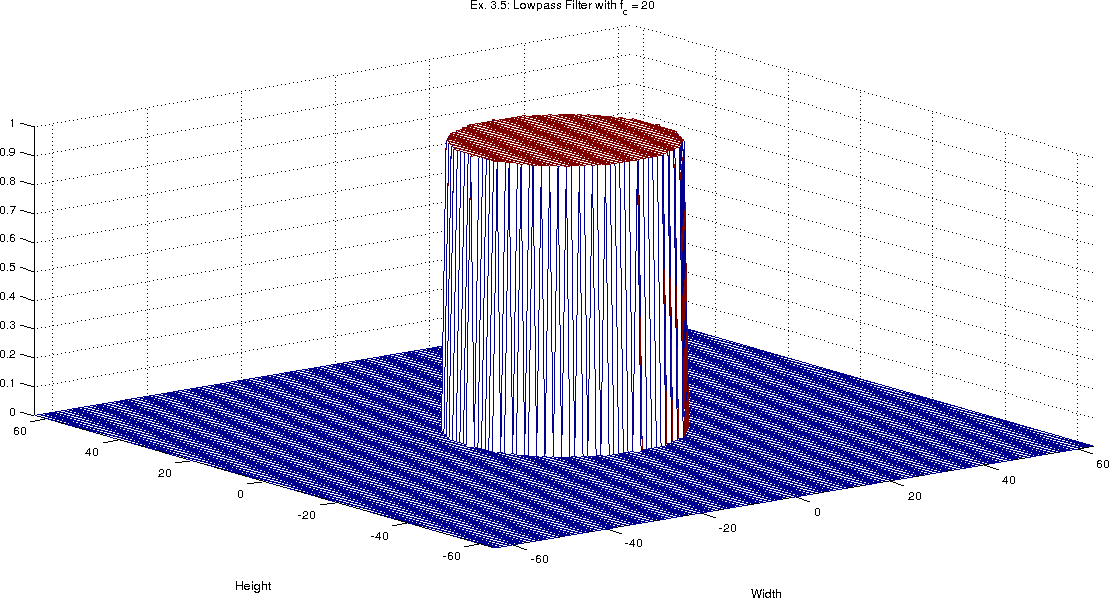
\includegraphics[width=0.70\textwidth]{images/ex_3_5_lowpass.png}
	\captionof{figure}{Lowpass Filter Mask with $f_c = 20$.}
	\label{fig:ex_3_5_lowpass}
\end{center}

\noindent Em seguida, o gráfico da frequência em magnitude, após a aplicação do filtro passa-baixo.
\begin{center}
	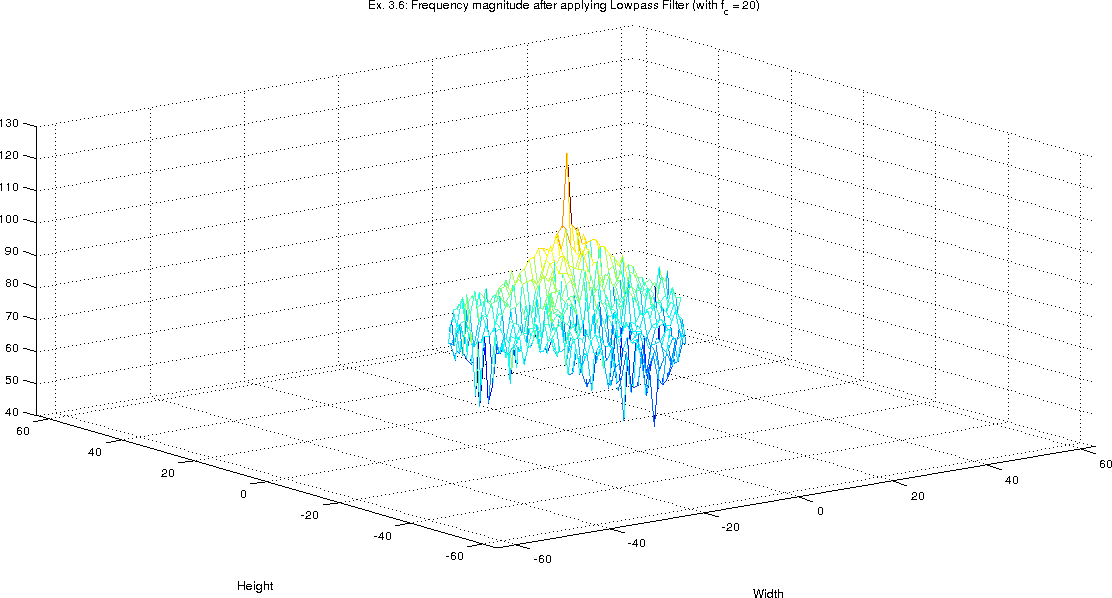
\includegraphics[width=0.70\textwidth]{images/ex_3_6_lowpass.png}
	\captionof{figure}{Frequency magnitude plot after applying a Lowpass Filter with $f_c = 20$.}
	\label{fig:ex_3_6_lowpass}
\end{center}

\clearpage

\noindent Após a aplicação das funções \texttt{ifft2} (e \texttt{ifftshift}), obtém-se a imagem resultante da aplicação do filtro.
\begin{center}
	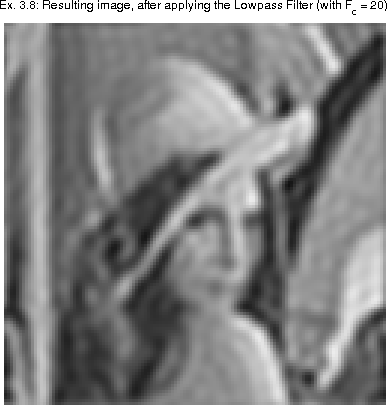
\includegraphics[width=0.20\textwidth]{images/ex_3_8_lowpass.png}
	\captionof{figure}{Resulting image, after applying a Lowpass Filter with $f_c = 20$.}
	\label{fig:ex_3_8_lowpass}
\end{center}

\clearpage

\noindent Apresenta-se em seguida a máscara criada para um filtro passa-alto, de frequência de corte $30$.
\begin{center}
	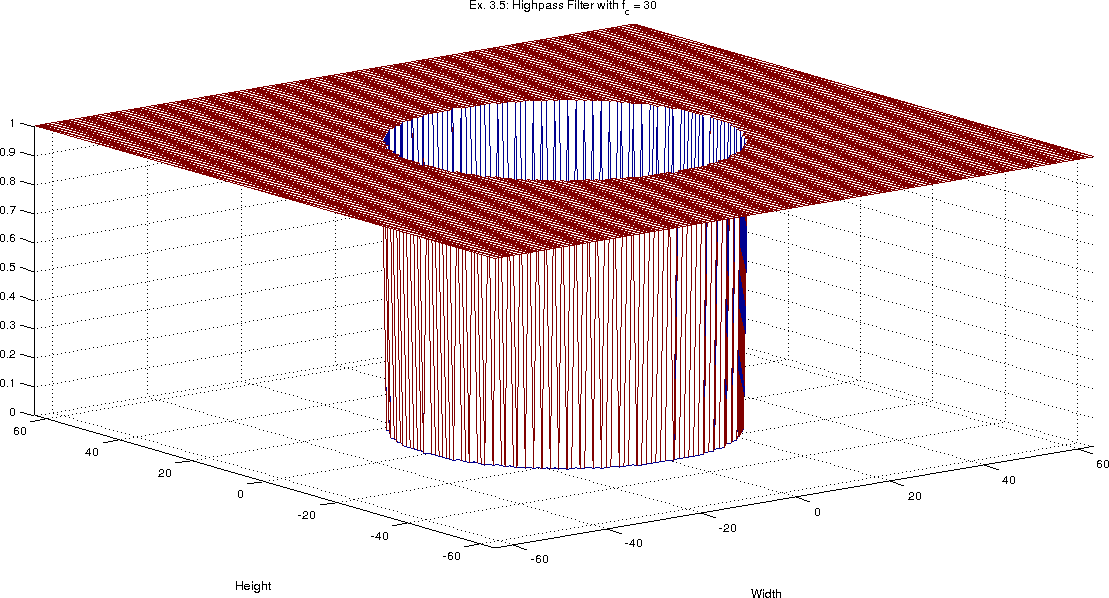
\includegraphics[width=0.70\textwidth]{images/ex_3_5_highpass.png}
	\captionof{figure}{Highpass Filter Mask with $f_c = 30$.}
	\label{fig:ex_3_5_highpass}
\end{center}

\noindent Em seguida, o gráfico da frequência em magnitude, após a aplicação do filtro passa-alto.
\begin{center}
	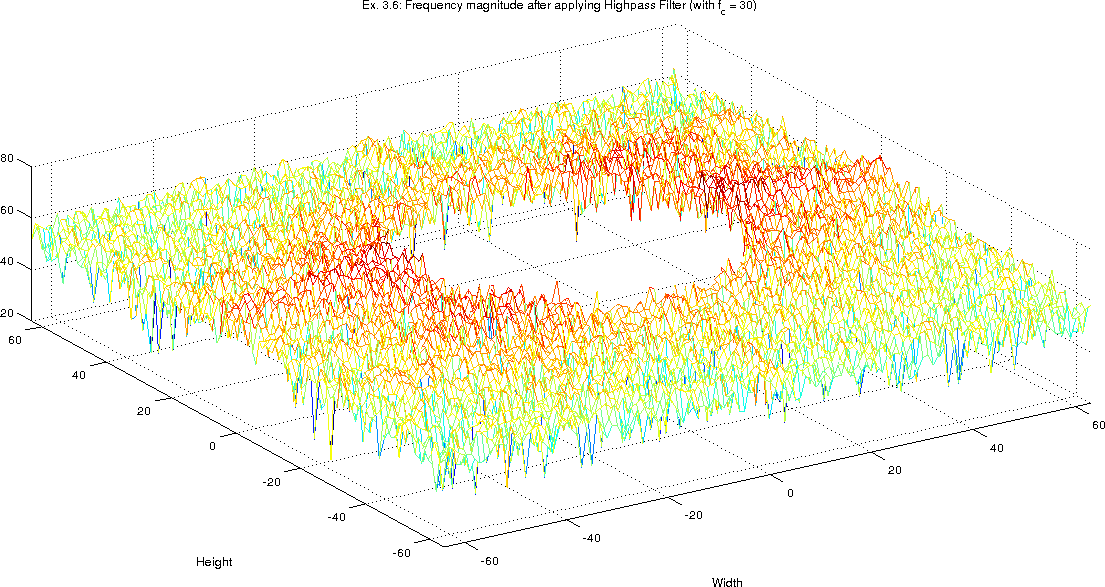
\includegraphics[width=0.70\textwidth]{images/ex_3_6_highpass.png}
	\captionof{figure}{Frequency magnitude plot after applying a Highpass Filter with $f_c = 30$.}
	\label{fig:ex_3_6_highpass}
\end{center}

\clearpage

\noindent Esta é a imagem resultante da aplicação desse filtro. Foi aumentado o contraste desta imagem (coeficiente de contraste de 10).
\begin{center}
	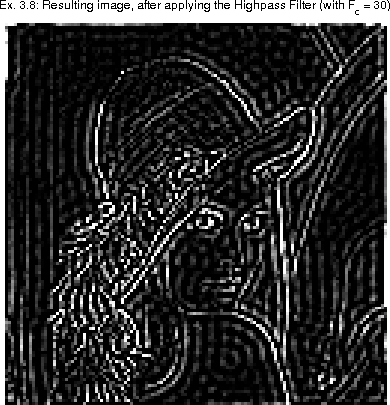
\includegraphics[width=0.20\textwidth]{images/ex_3_8_highpass.png}
	\captionof{figure}{Resulting image, after applying a Highpass Filter with $f_c = 30$ ($cc = 10$).}
	\label{fig:ex_3_8_highpass}
\end{center}

\subsection{Exercise 3.9}
\noindent As frequências baixas caracterizam as transições suaves de cor, enquanto que as frequências altas são responsáveis pelas mudanças abruptas. Como tal, após a aplicação de um filtro passa-baixo (i.e., que filtra as frequências acima de um determinado \emph{threshold}), a imagem resultante estará mais esbatida, com perda de algum detalhe. Já com a aplicação de um filtro passa-alto (i.e., que filtra as frequências abaixo de um determinado valor), a imagem resultante perderá as componentes responsáveis por grande parte da cor (como por exemplo, a componente $DC$) e, consequentemente, resultará numa imagem maioritariamente composta por contornos (frequências altas).

\clearpage
\section{Attachments}
\subsection{Trigonometric identities}
\label{subsec:trigident}
\noindent As simplicações da alínea \emph{\nameref{subsec:ex_1_1}} faz uso das seguintes igualdades:
\begin{equation}
	sin(\theta) \, cos(\varphi) = \frac{sin(\theta - \varphi) + sin(\theta + \varphi)}{2}
\end{equation}

\begin{equation}
	cos(-\theta) = cos(\theta)
\end{equation}

\end{document}
